Consider following unity gain feedback system. 
\begin{center}
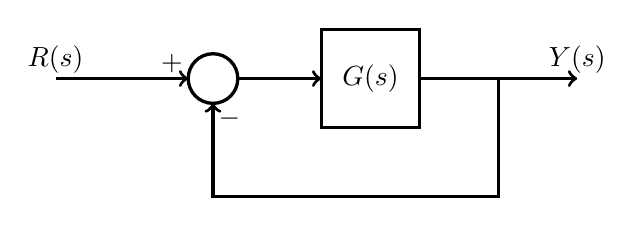
\begin{tikzpicture}[scale=1,inner sep=0pt,outer sep=0pt,very thick,
sysblock/.style={draw,rectangle,inner sep=2pt,minimum width=1.25cm,minimum height=1.25cm,inner sep=4pt, very thick}]
\draw (2,0) node[draw,circle] (sum1) {$\rule{0pt}{18pt}$};
%\draw (4,0) node[sysblock] (K) {$K$};
\draw (4,0) node[sysblock] (G) {$G(s)$};
\draw[->] (0,0) node[above=2pt] {$R(s)$} -- (sum1.180) node[above left=2pt] {$+$};
%\draw[->] (sum1.0)  -- (K.180);
%\draw[->] (K.0) -- (G.180);
\draw[->] (sum1.0) -- (G.180);
\draw[->] (G.0) -- ++(2,0) node[above=2pt] {$Y(s)$};
\draw[->] (G.0) ++(1,0) -- ++(0,-1.5) -| (sum1.-90) node[below right=2pt] {$-$};
\end{tikzpicture}
\end{center}
The Bode plot of $G(s)$ is shown below. $G(s)$ has all poles with negative real part,  except for a pole at $s=0$. \vspace{-.25in}
\begin{center}
%\includegraphics[width=4.5in]{./Problem08/bode3.pdf}
\includegraphics[width=4.5in]{\mainfolder/LectureNotes/\lecturefolder/HomeworkProblems/Problem10/bode3.pdf}

\end{center}\vspace{-.25in}
\begin{enumerate}[(a)]
\item Sketch the Nyquist plot and determine if the feedback system is closed loop stable. For full credit, your sketch must accurately reflect which quadrants the Nyquist plot enters, and the number of encirclements of $-1+j0$.
\item If stable, find the phase and gain margins for this feedback control system.
\end{enumerate}